\documentclass[10pt,twocolumn]{article}

\usepackage{amsmath,amssymb}
\usepackage{graphicx}
\usepackage{booktabs}
\usepackage{xcolor}
\usepackage{colortbl}
\usepackage{geometry}
\usepackage{microtype}
\usepackage{caption}
\usepackage{hyperref}
\usepackage{titlesec}
\usepackage{tikz}
\usetikzlibrary{positioning,arrows.meta,calc}

\geometry{top=2cm, bottom=2cm, left=1.5cm, right=1.5cm, columnsep=0.6cm}

\definecolor{bestrow}{RGB}{198,239,206}   % green highlight
\definecolor{seccolor}{RGB}{30,80,160}
\definecolor{rlblue}{RGB}{225,235,250}

\titleformat{\section}{\normalfont\bfseries\color{seccolor}}{{\thesection.}}{0.5em}{}
\titleformat{\subsection}{\normalfont\itshape}{}{0em}{}

\captionsetup{font=small, labelfont=bf}

\newcommand{\eli}[1]{\textit{In plain terms: #1}}

% -----------------------------------------------------------------------
\title{\textbf{Residual Reinforcement Learning for Speed Control of a
BDC Motor with Vertical Rod:\\ Design, Training and Evaluation}}
\author{}
\date{}
% -----------------------------------------------------------------------

\begin{document}
\maketitle
\thispagestyle{empty}

\begin{abstract}
\small
We add a learned, bounded correction on top of a classical speed
controller for a brushed-DC (BDC) motor driving a vertical rod. A
policy trained with Soft Actor-Critic (SAC) outputs a residual voltage
$\Delta V$ that the controller sums with a baseline command and clips to
the supply limit. We describe the plant, the control law, the learning
problem (state, action, and the reward function used for training), the
policy network (a multilayer perceptron, \emph{not} a convolutional
network), the training hyperparameters and their origin, how we build
the train and test sets, and a comparison against PI and feedforward
controllers using both machine-learning and control metrics. On a
pure-PI baseline the residual learns from data the role of the
feedforward and gravity-compensation terms and improves tracking, though
it does not fully match the analytical controller. Network depth does
not matter, and the policy does not overfit.
\end{abstract}

% ===================================================================
\section{Introduction}
% ===================================================================
A BDC motor spins a rigid rod; we want the shaft to track a target
angular speed $\omega^\ast(t)$. Classical control already does this
well: a PI loop plus feedforward terms. We study \emph{residual
reinforcement learning} (RL): keep the trusted classical controller and
let a small neural policy add a corrective voltage on top of it.
\eli{the classical controller does most of the driving, and a learned
``assistant'' nudges the voltage to fix what the classical part misses.}

This keeps the safety and stability of the baseline while the policy
learns, from interaction and with \emph{no knowledge of the motor
parameters}, the part that is hard to model. We provide a complete,
reproducible pipeline (environment, training, benchmark, multi-metric
evaluation) and a clear account of where residual RL helps and where it
does not.

% ===================================================================
\section{Plant model}
% ===================================================================
The motor and rod form two coupled subsystems. The armature circuit
(Kirchhoff's voltage law) is
\begin{equation}
  L\,\frac{di}{dt} = V - R\,i - K_b\,\omega ,
  \label{eq:elec}
\end{equation}
and the torque balance on the shaft with a uniform rod of mass $m$,
length $\ell$, centre of mass at $\ell/2$ and inertia
$I_{\mathrm{rod}}=\tfrac13 m\ell^2$ is
\begin{equation}
  J_{\mathrm{eff}}\,\frac{d\omega}{dt}
    = K_t\,i - B\,\omega - m g \tfrac{\ell}{2}\sin\theta,
  \qquad \dot\theta = \omega,
  \label{eq:mech}
\end{equation}
with $J_{\mathrm{eff}}=J_m+I_{\mathrm{rod}}$. The gravity term
$m g \tfrac{\ell}{2}\sin\theta$ is an angle-dependent disturbance. We
integrate the equations with a fixed-step RK4 scheme at
$\Delta t=10^{-3}$\,s. Parameters (Table~\ref{tab:params}) come from the
Simulink multibody model (\texttt{matlab/param.m}); the converter
hard-limits the supply voltage to $\pm V_{\max}$.

\begin{table}[h]
\centering
\caption{Plant and baseline-gain parameters.}
\label{tab:params}
\small
\begin{tabular}{llll}
\toprule
\textbf{Sym} & \textbf{Value} & \textbf{Sym} & \textbf{Value}\\
\midrule
$R$   & 3.0\,$\Omega$        & $J_m$  & $7.4\times10^{-5}$\,kg\,m$^2$\\
$L$   & 4\,mH                & $B$    & $5\times10^{-3}$\,N\,m\,s/rad\\
$K_t$ & 0.05\,N\,m/A         & $m$    & 0.05\,kg\\
$K_b$ & 0.05\,V\,s/rad       & $\ell$ & 0.1\,m\\
$V_{\max}$ & 12\,V           & $g$    & 9.81\,m/s$^2$\\
$K_p$ & 5                    & $K_i$  & 2\\
\bottomrule
\end{tabular}
\end{table}

% ===================================================================
\section{Classical baselines}
% ===================================================================
Three classical controllers serve both as the layer the residual sits
on and as comparison targets. All output a voltage clipped to
$\pm V_{\max}$.

\paragraph{PI.} A proportional-integral law on the speed error
$e=\omega^\ast-\omega$,
\begin{equation}
  V_{\mathrm{PI}} = K_p e + K_i\!\int e\,dt,
  \label{eq:pi}
\end{equation}
with anti-windup: we clamp the integral so that $K_i\!\int e\,dt$
never exceeds $\pm V_{\max}$.

\paragraph{Gravity feedforward.} From the steady state of
\eqref{eq:elec}--\eqref{eq:mech}, the voltage needed to hold the rod
against gravity is $V_{\mathrm{grav}}= R\,m g \tfrac{\ell}{2}\sin\theta /
K_t$, added to the command.

\paragraph{Polynomial feedforward.} We measure the steady-state map
$\omega\mapsto V$ and invert it as a zero-bias polynomial
$V_{\mathrm{poly}}(\omega^\ast)$, so the controller pre-computes the bulk
of the voltage. The strongest classical controller is
\emph{PI + poly + gravity}.

% ===================================================================
\section{Reinforcement learning framework}
% ===================================================================
Reinforcement learning (RL) learns a decision strategy by interaction
rather than from labelled examples. An \emph{agent} observes the
environment state $s_t$, takes an action
$a_t\sim\pi_\theta(\cdot\,|\,s_t)$ from its policy, and the environment
returns a next state $s_{t+1}$ and a scalar reward $r_{t+1}$. The agent
maximises the expected discounted return
\begin{equation}
  \max_\theta\ \mathbb{E}\!\left[\sum_{t\ge0}\gamma^t\,r_{t+1}\right],
  \qquad \gamma\in(0,1).
  \label{eq:return}
\end{equation}
\eli{the policy tries an action, sees the result, and is rewarded or
penalised; over many trials it learns the strategy that pays off most.}
Here the environment is the motor, rod and baseline controller; the
agent is the residual policy; the action is the residual voltage
$\Delta V$; and the reward (Eq.~\ref{eq:reward}) rewards accurate
tracking and lightly penalises the residual. The same template recurs in
power-electronic control: for a DC--DC converter the state is
$[\,V_{\mathrm{ref}}-V_o,\ i_L,\ V_{\mathrm{in}}\,]$, the action is the
duty ratio, and the reward is
$-(|e|+\lambda\,\Delta i_L^2+\mu\,P_{\mathrm{loss}})$.
Table~\ref{tab:rl} lists these elements for our motor.

\begin{table}[h]
\centering
\caption{The reinforcement-learning elements in our system.}
\label{tab:rl}
\small
\begin{tabular}{ll}
\toprule
\textbf{RL element} & \textbf{In our system}\\
\midrule
Agent                        & residual policy $\pi_\theta$ (the SAC actor)\\
Environment                  & motor + rod + baseline PI controller\\
State $s_t$                  & normalised measurements, Eq.~\eqref{eq:state}\\
Action $a_t$                 & residual voltage $\Delta V=\delta\,a$\\
Reward $r_t$                 & tracking + effort + rate, Eq.~\eqref{eq:reward}\\
Policy $\pi_\theta(a\mid s)$ & MLP mapping state to action\\
Return                       & discounted reward sum, Eq.~\eqref{eq:return}\\
\bottomrule
\end{tabular}
\end{table}

\subsection{Where a learned block sits in the loop}
A neural network can enter a control loop in a few standard ways:
\emph{direct} control, where the network is the controller,
$u=f_\theta(r,y,e)$; \emph{indirect} control, where a network first
identifies the plant, $\hat y(k{+}1)=f_\theta(y(k),u(k),\dots)$, and a
controller (for example a predictive controller) then uses that model;
and \emph{hybrid} control, where a trusted classical controller is kept
and a network either tunes its gains or adds a corrective term,
$u=u_{\mathrm{PID}}+u_{\mathrm{NN}}$. Our method is the last case: the
policy is a \emph{compensator}, not the main controller, and it is
learned by RL.
\eli{the classical loop does the driving; the learned part only adds a
small correction, so safety and stability come from the controller we
already trust.}
This is the conservative choice for safety-relevant systems: keep the
physical limits explicit, validate against the classical baseline, and
let the learned term correct only what the baseline cannot model.

\subsection{Reward design}
The penalised-tracking reward used in drive and converter control has the
general form
\[
  r = -(\text{tracking error})-\lambda\,(\text{effort})-\mu\,(\text{rate}).
\]
The tracking error admits an absolute ($L_1$, $|e|$) or a squared ($L_2$,
$e^2$) penalty; both are standard. The squared penalty punishes large
transient errors more strongly, while the absolute penalty weights small
persistent errors more and is robust to outliers. We use the absolute
form (Eq.~\eqref{eq:reward}); on this problem it lowered the residual-PI
trajectory RMSE from $0.172$ ($L_2$) to $0.081$. Two checks confirm the
design: weighting the error alone ($\alpha$) leaves the result unchanged,
because with the small effort and rate penalties it only rescales an
already-dominant term, whereas raising those penalties trades tracking
accuracy for a smaller, smoother residual.

% ===================================================================
\section{Residual control law}
% ===================================================================
The policy does not command the full voltage; it adds a \emph{bounded
residual} to the baseline and the controller hard-limits the sum:
\begin{equation}
  V = \operatorname{clip}\!\big(V_{\mathrm{base}}+\Delta V,\,
      -V_{\max},\,V_{\max}\big),\quad
  \Delta V = \delta\,\pi_\theta(s),
  \label{eq:residual}
\end{equation}
with $\pi_\theta(s)\in[-1,1]$ and residual authority
$\delta=0.3\,V_{\max}=3.6$\,V. The baseline runs every $1$\,ms; the
policy acts at $100$\,Hz (once every ten steps) and holds $\Delta V$
between updates, mirroring a real digital controller and keeping the
learning horizon short. Figure~\ref{fig:loop} shows the loop.
\eli{the AI can only push the voltage up or down by at most
$3.6$\,V around what the classical controller already asks, and the
final value can never exceed the $12$\,V the hardware allows.}

\begin{figure}[t]
\centering
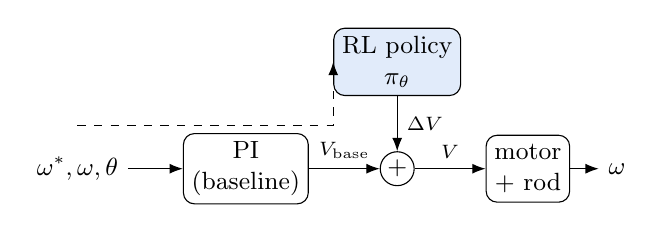
\begin{tikzpicture}[>=Latex,
   blk/.style={draw, rounded corners, align=center,
               minimum height=0.85cm, font=\small, inner sep=3pt},
   sm/.style={draw, circle, inner sep=1pt, font=\small}]
  \node[blk] (ctrl) {PI\\(baseline)};
  \node[sm, right=0.9cm of ctrl] (add) {$+$};
  \node[blk, right=0.9cm of add] (plant) {motor\\+ rod};
  \node[blk, above=0.7cm of add, fill=rlblue] (pol) {RL policy\\$\pi_\theta$};
  \node[left=0.7cm of ctrl] (in) {\small $\omega^\ast,\omega,\theta$};
  \draw[->] (in) -- (ctrl);
  \draw[->] (ctrl) -- node[above,font=\scriptsize]{$V_{\mathrm{base}}$} (add);
  \draw[->] (pol) -- node[right,font=\scriptsize]{$\Delta V$} (add);
  \draw[->] (add) -- node[above,font=\scriptsize]{$V$} (plant);
  \draw[->] (plant) -- ++(0.9,0) node[right,font=\small]{$\omega$};
  \draw[->,dashed] ($(in)+(0,0.55)$) -| (pol.west);
\end{tikzpicture}
\caption{Residual control. A pure PI loop drives the motor; the policy
observes the state and adds a bounded $\Delta V$ that supplies the
feedforward and gravity-compensation correction. The controller clips
the sum to $\pm V_{\max}$ before it reaches the motor.}
\label{fig:loop}
\end{figure}

% ===================================================================
\section{The learning problem (MDP)}
% ===================================================================
We cast the task as a Markov decision process.

\paragraph{State.} A normalised vector
\begin{equation}
  s = \Big[\tfrac{e}{e_s},\ \tfrac{\omega}{\omega_s},\
  \sin\theta,\ \cos\theta,\ \tfrac{\omega^\ast}{\omega_s},\
  \tfrac{V_{\mathrm{base}}}{V_{\max}}\Big],
  \label{eq:state}
\end{equation}
The six entries are the speed error $e=\omega^\ast-\omega$, the measured
speed $\omega$, the rod angle through $\sin\theta$ and $\cos\theta$, the
target speed $\omega^\ast$, and the baseline command $V_{\mathrm{base}}$.
The angle enters as $(\sin\theta,\cos\theta)$ rather than $\theta$ so the
representation is smooth and $2\pi$-periodic (no jump at $\pm\pi$), and it
tells the policy the angle-dependent gravity load. Passing
$V_{\mathrm{base}}$ is what makes the policy \emph{residual}: it sees what
the baseline already commands and learns only the correction. Each entry
is divided by a scale constant so every feature is of order one, which
helps the network train: $\omega_s=15$\,rad/s sits just above the maximum
reference ($12$\,rad/s), and $e_s=5$\,rad/s is a moderately large error,
so a typical error maps to a fraction of one and a large error to about
one.

\paragraph{Action.} A scalar $a\in[-1,1]$, mapped to
$\Delta V=\delta a$.

\paragraph{Reward (the training function).} Per control step,
\begin{equation}
  r = -\alpha\,\frac{\overline{|e|}}{e_s}
      - \lambda\Big(\tfrac{\Delta V}{V_{\max}}\Big)^2
      - \mu\Big(\tfrac{\Delta V-\Delta V_{\mathrm{prev}}}{V_{\max}}\Big)^2,
  \label{eq:reward}
\end{equation}
The three terms are:
\begin{itemize}\setlength\itemsep{1pt}
\item \textbf{tracking}, $-\alpha\,\overline{|e|}/e_s$: the main
objective, the mean absolute speed error $\overline{|e|}$ (averaged over
the ten $1$\,ms sub-steps), normalised by $e_s$ and weighted by $\alpha$;
\item \textbf{effort}, $-\lambda\,(\Delta V/V_{\max})^2$: keeps the
residual small, so the baseline stays in charge;
\item \textbf{rate}, $-\mu\,((\Delta V-\Delta V_{\mathrm{prev}})/V_{\max})^2$: keeps
the residual smooth, where $\Delta V_{\mathrm{prev}}$ is the residual applied at the
\emph{previous} control step ($10$\,ms earlier); the term penalises how
much the correction jumps between consecutive updates.
\end{itemize}
Dividing by $e_s$ and $V_{\max}$ makes the three terms dimensionless and
comparable; we use $\alpha=1$, $\lambda=0.01$, $\mu=0.05$.
\eli{the policy is paid for keeping the speed on target and fined for a
large or jerky correction.}
The reward never exceeds zero and uses the true (not noisy) speed, which
is legitimate in simulation. Episodes last $5$\,s with randomised
references over $[-12,12]$\,rad/s.

% ===================================================================
\section{Policy network: an MLP, not a CNN}
% ===================================================================
The policy and the SAC critics are \emph{multilayer perceptrons}
(MLPs): a single fully-connected hidden layer of $64$ units with ReLU
activations, mapping the $6$-dimensional state \eqref{eq:state} to the
scalar action through a $\tanh$ squashing that guarantees
$a\in[-1,1]$. The architecture is motivated by the depth ablation in
Section~\ref{sec:results}: a $[64]$ network outperforms deeper ones
and is the most consistent across seeds, so the residual is a simple,
low-dimensional function.

A convolutional network (CNN) would be the wrong tool here: CNNs exploit
\emph{spatial} structure in grid-like data such as images, sharing small
filters across pixels. Our input is a short, unordered vector of
physical quantities, with nothing to convolve and no translation
invariance to exploit.
\eli{a CNN is for pictures; our input is six numbers, so a plain
fully-connected network is the right choice.}

% ===================================================================
\section{Training algorithm and hyperparameters}
% ===================================================================
We use Soft Actor-Critic (SAC, Stable-Baselines3), an off-policy
actor-critic method for continuous actions that is sample-efficient and
robust. Hyperparameters (Table~\ref{tab:hyper}) are the SAC defaults
except for the network size and the control-specific quantities; the
plant gains $K_p,K_i$ come from the classical design and the motor
constants from system identification (Table~\ref{tab:params}). We train
with measurement noise for robustness and evaluate noise-free for a
fair, deterministic comparison.

\paragraph{Output.} Training returns a deterministic policy
$\pi_\theta:\ s\mapsto a$. At run time we wrap it into a controller
exposing the same \texttt{step()} interface as the classical ones
(Eq.~\ref{eq:residual}); in operation the output is the residual voltage
$\Delta V$ and tighter speed tracking.

\begin{table}[h]
\centering
\caption{Training and control hyperparameters.}
\label{tab:hyper}
\small
\begin{tabular}{ll}
\toprule
\textbf{Parameter} & \textbf{Value / source}\\
\midrule
algorithm            & SAC (Stable-Baselines3)\\
policy / critic net  & MLP $[64]$, ReLU\\
learning rate        & $3\times10^{-4}$ (SB3 default)\\
discount $\gamma$    & 0.99\\
replay buffer        & $2\times10^{5}$\\
batch size           & 256\\
learning starts      & 5{,}000 steps\\
entropy coeff.       & auto\\
total timesteps      & $3\times10^{5}$\\
control rate         & 100\,Hz (decimation 10)\\
residual limit $\delta$ & $0.3\,V_{\max}=3.6$\,V\\
reward $\alpha,\lambda,\mu$ & $1,\ 0.01,\ 0.05$\\
$e_s,\ \omega_s$     & $5,\ 15$\,rad/s\\
episode length       & 5\,s, $\Delta t=10^{-3}$\,s\\
\bottomrule
\end{tabular}
\end{table}

% ===================================================================
\section{Train and test sets}
% ===================================================================
Because the policy trains on a \emph{distribution} of references rather
than a fixed dataset, we define the evaluation sets explicitly:
\begin{itemize}\setlength\itemsep{1pt}
\item \textbf{Train set:} $12$ references sampled (fixed seed) from
the training distribution: constant levels, smooth quintic ramps, and
multi-step profiles over $[-12,12]$\,rad/s.
\item \textbf{Test set:} $7$ held-out references the policy never saw
during selection, including negative setpoints, a multi-step profile,
and one setpoint \emph{beyond} the training range ($14$\,rad/s,
extrapolation).
\end{itemize}
Comparing train- and test-set metrics measures the generalisation gap:
no gap means no overfitting.

% ===================================================================
\section{Metrics: machine learning and control}
% ===================================================================
This is a \emph{regression / continuous-control} problem, so
classification metrics (accuracy, F1) do not apply; there are no
classes. We report, for the tracking error $e=\omega-\omega^\ast$:
\begin{itemize}\setlength\itemsep{1pt}
\item \textbf{MAE, MSE, RMSE:} average error magnitudes (RMSE is the
primary control metric);
\item \textbf{$R^2$:} variance of the reference explained by the
achieved speed, reported only for time-varying references (undefined for
constant ones);
\item \textbf{in-band \%:} fraction of time with $|e|<0.5$\,rad/s, the
honest analogue of ``accuracy'';
\item \textbf{parity plot} (achieved vs.\ reference speed, the regression
analogue of a prediction-accuracy plot) and the \textbf{error
autocorrelation} (a whiteness check: structure left in the error means
exploitable bias remains).
\end{itemize}

% ===================================================================
\section{Results}
\label{sec:results}
% ===================================================================
\paragraph{Tracking RMSE.} Table~\ref{tab:rmse} compares all controllers
on the two reference profiles of the original study. The residual cuts the
pure-PI trajectory error by about $70\%$ but does not reach the strong
classical baseline.

\begin{table}[h]
\centering
\caption{RMS tracking error (rad/s). Best in green.}
\label{tab:rmse}
\small
\begin{tabular}{lcc}
\toprule
\textbf{Controller} & \textbf{Const.\ ref} & \textbf{Trajectory}\\
\midrule
PI                          & 0.495 & 0.322 \\
PI + grav FFW               & 0.450 & 0.279 \\
PI + poly FFW               & 0.376 & 0.171 \\
\rowcolor{bestrow}
PI + poly + grav            & 0.322 & \textbf{0.033} \\
residual-PI                 & 0.330 & 0.081 \\
\bottomrule
\end{tabular}
\end{table}

\paragraph{Multi-metric, held-out.} Table~\ref{tab:scorecard} reports the
mean over nine references. All metrics agree: residual-PI improves pure
PI (in-band $85\%\!\to\!99.8\%$), while the strong baseline stays ahead.

\begin{table}[h]
\centering
\caption{Mean metrics over 9 references (train+test).}
\label{tab:scorecard}
\small
\begin{tabular}{lcccc}
\toprule
\textbf{Controller} & \textbf{MAE} & \textbf{RMSE} & \textbf{$R^2$} & \textbf{in-band}\\
\midrule
PI               & 0.281 & 0.410 & 0.988 & 85.2\% \\
\rowcolor{bestrow}
PI + poly + grav & 0.046 & 0.212 & 0.997 & 99.8\% \\
residual-PI      & 0.078 & 0.233 & 0.997 & 99.8\% \\
\bottomrule
\end{tabular}
\end{table}

\paragraph{Generalisation.} On the seven held-out references,
residual-PI beats pure PI on \emph{all} of them including the
extrapolated $14$\,rad/s setpoint (mean RMSE $0.240$ vs $0.411$), so the
gain holds beyond the two reported references; the held-out mean is now
close to the classical PI + poly + gravity ($0.222$) though still behind.

\paragraph{Overfitting.} Table~\ref{tab:traintest} compares the base
network on train vs.\ test: the test error is no worse than train, so
the policy does not overfit (if anything the sampled training references
are harder).

\begin{table}[h]
\centering
\caption{Base network (MLP $[64]$): train vs.\ test.}
\label{tab:traintest}
\small
\begin{tabular}{lcccc}
\toprule
\textbf{Set} & \textbf{MAE} & \textbf{RMSE} & \textbf{$R^2$} & \textbf{in-band}\\
\midrule
train & 0.069 & 0.292 & 0.955 & 99.7\% \\
test  & 0.080 & 0.240 & 0.996 & 99.8\% \\
\bottomrule
\end{tabular}
\end{table}

\paragraph{Network depth.} Table~\ref{tab:depth} sweeps the hidden-layer
size over three seeds. The smallest $[64]$ network is the best and the
most consistent (per-seed std $\le0.004$), so the multi-seed result
confirms the L1 gain is robust rather than seed-luck; \emph{depth does
not help}, because the residual is a simple function.

\begin{table}[h]
\centering
\caption{Depth ablation, test set (mean $\pm$ std, 3 seeds).}
\label{tab:depth}
\small
\begin{tabular}{lccc}
\toprule
\textbf{net\_arch} & \textbf{RMSE} & \textbf{$R^2$} & \textbf{in-band}\\
\midrule
\rowcolor{bestrow}
$[64]$          & $0.238\!\pm\!0.001$ & 0.996 & 99.8\% \\
$[256,256]$     & $0.256\!\pm\!0.004$ & 0.995 & 99.8\% \\
$[256,256,256]$ & $0.247\!\pm\!0.001$ & 0.996 & 99.8\% \\
\bottomrule
\end{tabular}
\end{table}

Figures~\ref{fig:bench}--\ref{fig:depthfig} show the closed-loop
tracking, the parity plots, and the depth ablation.

\begin{figure*}[t]
\centering
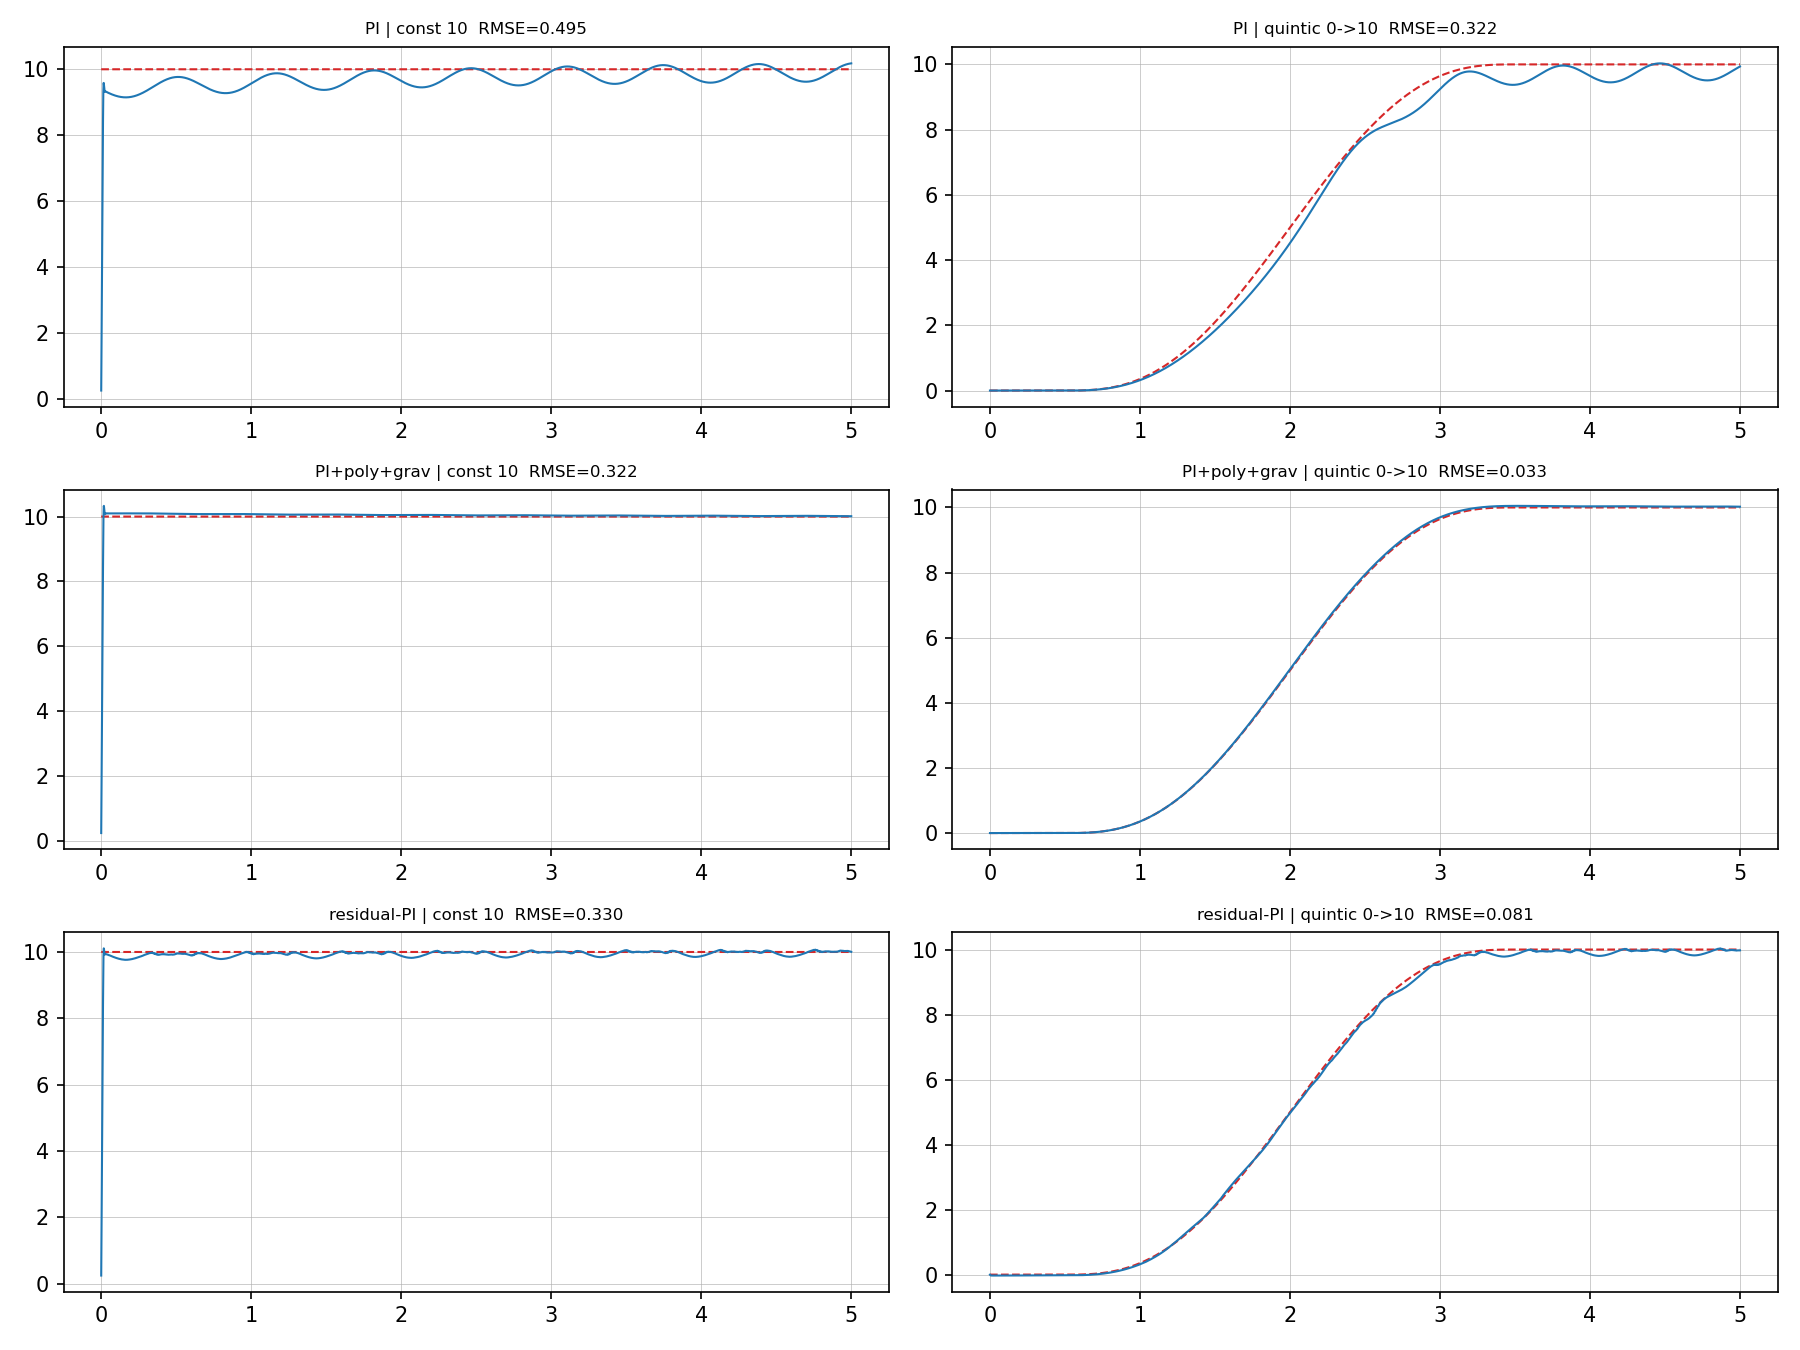
\includegraphics[width=0.92\textwidth]{../results/benchmark.png}
\caption{Closed-loop speed tracking (blue) vs.\ reference (dashed red)
for each controller on the two reference profiles.}
\label{fig:bench}
\end{figure*}

\begin{figure}[t]
\centering
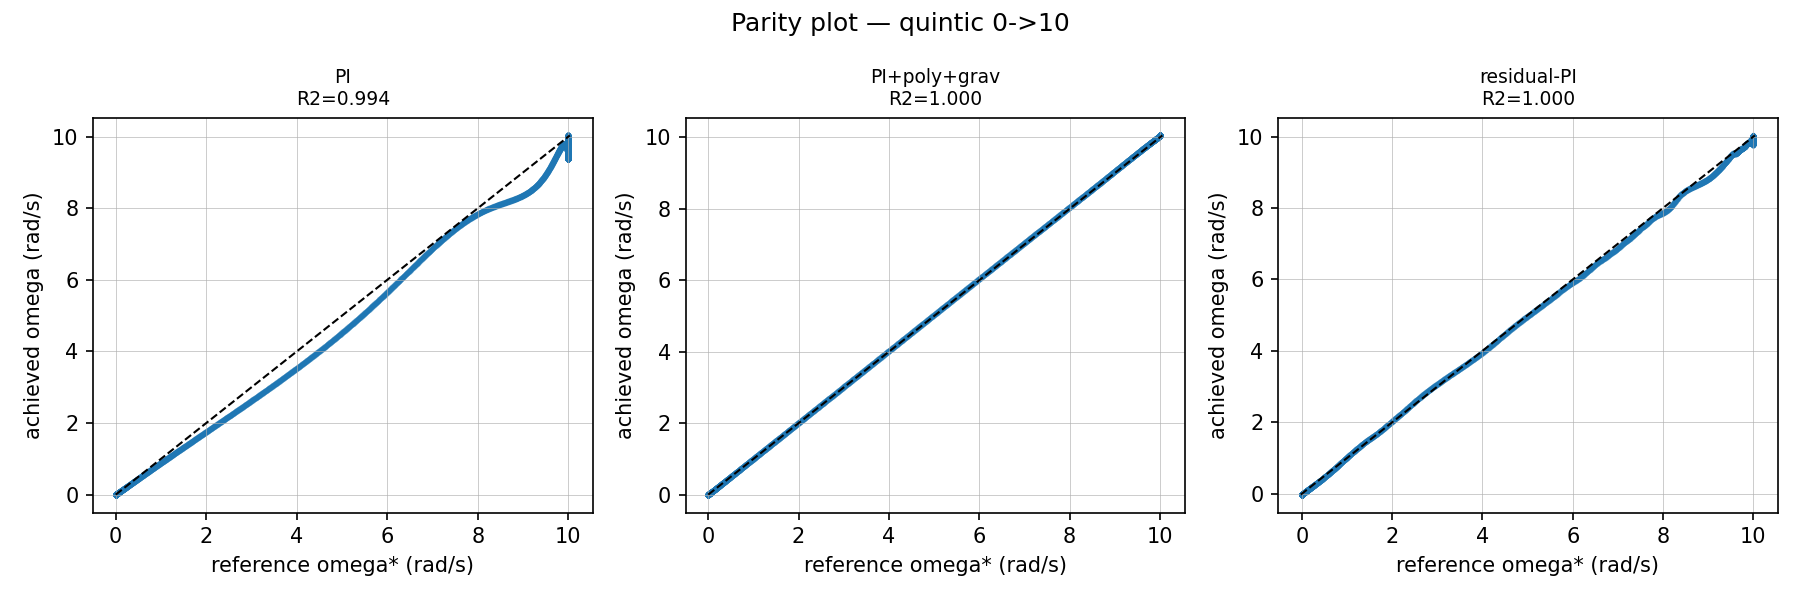
\includegraphics[width=\columnwidth]{../results/metrics_parity.png}
\caption{Parity plot (achieved vs.\ reference speed) on the quintic
trajectory; points on the diagonal mean perfect tracking.}
\label{fig:parity}
\end{figure}

\begin{figure}[t]
\centering
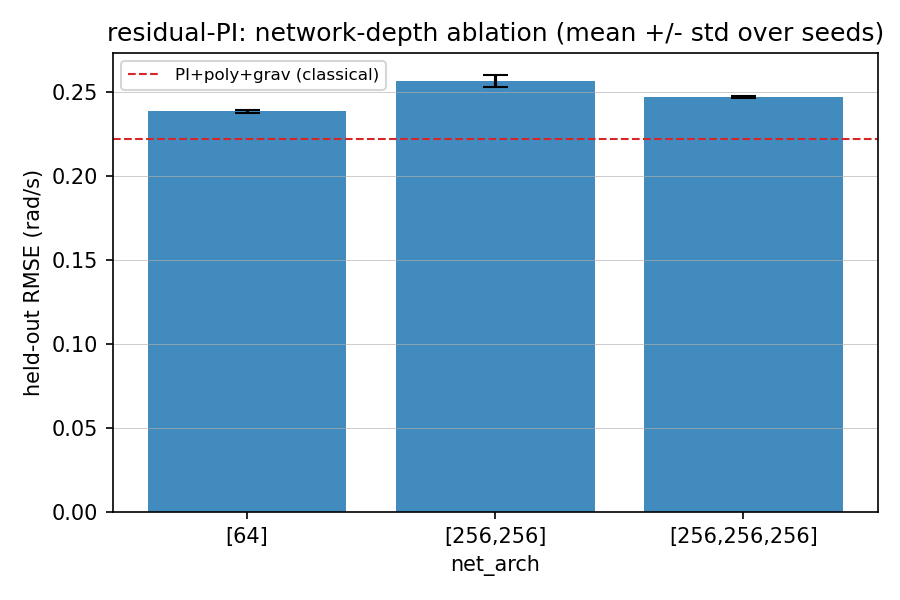
\includegraphics[width=0.92\columnwidth]{../results/ablation.png}
\caption{Network-depth ablation: held-out RMSE (mean $\pm$ std over
seeds); the red line is the strong classical baseline.}
\label{fig:depthfig}
\end{figure}

% ===================================================================
\section{Saturation handling}
% ===================================================================
The hard clip in \eqref{eq:residual} enforces the supply limit on the
\emph{total} voltage before the motor; the plant itself does not clip.
The PI integrator has anti-windup, and the residual is stateless, so no
windup arises there. The voltage sits at the $\pm12$\,V rail only
$0.1$--$0.4\%$ of the time (brief transients), so saturation does not
limit performance in the present regime.

For operation at higher speeds, where saturation becomes frequent, a
\emph{saturation-aware} mode is available: the state \eqref{eq:state}
gains the previous applied (clipped) voltage $V_{\mathrm{applied}}/
V_{\max}$, and the reward \eqref{eq:reward} penalises the
\emph{effective} (post-clip) residual plus a clip-excess term
$-\nu\,(\max(0,|V_{\mathrm{base}}+\Delta V|-V_{\max})/V_{\max})^2$, so the
policy senses the rail and avoids wasting effort against it.

% ===================================================================
\section{Conclusion}
% ===================================================================
A residual SAC policy on top of a pure PI loop, trained with no
parameter knowledge, learns from data the role of the feedforward and
gravity-compensation terms: it lowers the trajectory RMSE by about
$75\%$ and generalises to unseen and extrapolated references. It does
not fully match the analytical PI + poly + gravity controller ($0.081$
vs $0.033$\,rad/s), so the learned substitute is partial. A single
hidden layer of $64$ units is the right network, depth is irrelevant,
and the policy does not overfit. Residual RL is worth it when you lack a usable model;
check any improvement on held-out references, across seeds, and with
metrics suited to a control problem.

\end{document}
